\chapter{Getting started} \label{GetStarted}

\section{Installation}

\dfastbe has been developed using Python, but it's distributed as a binary.
It consists of one executable called 'dfastbe.exe' and a large number of supporting libraries and some configuration files.
The program can be run as a command line tool performing either the bank line detection step (see \autoref{Sec:rundetect}) or the bank erosion (see \autoref{Sec:runbank}) step, or in a graphical mode which can be used to edit the analysis settings and run the analysis.

By default \dfastbe is looking for the definition file 'dfastbe.cfg' in the current work directory.
When the definition file has another name or location, this should be passed when the modules are called.

\section{Scenario plan}

\dfastbe is not calibrated for local bank erosion\footnote{This is almost impossible, due to other uncertainties in bank properties, limited availability of field data of measured bank erosion and the fact that the simulation models have been designed for longer river reaches.
Locally \dfastbe could be calibrated when historical data of bank erosion is available.
However, this does not automatically imply that \dfastbe would give good results a few kilometers further downstream with the same settings, because the bank properties can be completely different.}.
Therefore it is strongly advised to use \dfastbe only in a \emph{relative} way.
In this way an image can be formed of

\begin{itemize}
\item at which locations the bank is most sensitive to erosion (by comparing different locations along the river)
\item how sensitive a location is for certain measures (by comparing different scenarios at one location)
\end{itemize}

We advise to compute different scenarios and compare between them.
An example is: 1 scenario with a subsoil of sand and 1 scenario with a subsoil of clay.
This means that only the type of subsoil is changed and the other input remains unchanged.

\section{Steady-state hydrodynamic simulations}

Before \dfastbe can be used, steady state hydrodynamic computations have to be performed for each discharge level.
\dfastbe supports results coming from \dflowfm and, after a conversion step, results coming from \dflow and WAQUA\footnote{\dflowfm and WAQUA models and Baseline schematisations of the Dutch river system can be requested via Helpdeskwater.nl Onderwerpen > Applicaties en modellen > Water en ruimte > Gebiedsschematisaties > Servicedesk > Meldingsformulier}.
This first requires a schematisation of the discharge hydrograph in discharge levels and a probability per discharge step.
The discretisation of the discharge hydrograph is not a trivial procedure.
Deltares advises to use at least ten discharge levels.

By default two figures are generated during \dfastbe computation which the user can use to check if the discharge levels are chosen properly.
These are a figure with water levels and a figure with flow velocities.
In both figures the area that is sensitive to erosion is indicated by means of bank levels and protection levels, and critical flow velocities respectively.
Based on these figures it can be decided to include or remove discharge levels from the computation.
For each discharge level a netCDF map-file (\dflowfm output file) must be provided -- if \dflow or WAQUA simulation results are available the TRIM- or SDS-files need to be converted to a netCDF map-file mimicking the \dflowfm output.
\dfastbe uses the water levels and flow velocities that are stored in the last time step.
It is important that the hydrodynamic computations are in steady state -- only the last time step of each simulation output file is used.
The probability (normalized weighting of the time period) per discharge level is defined by the user in the configuration file.

\Note It is of utmost importance that in the netCDF map-file with the reference (average) discharge (which is used to establish the initial bank lines) the water remains within the main channel during the whole computation.
Practically this means that the simulation has to be started with a low initial water level with no (or as little as possible) water in the flood plains.
When this criterion is not met, the bank line detection algorithm may incorrectly identify bank lines when water is unable to recede from depressions in the flood plain.

An example of discharge levels for the river Meuse in combination with different probabilities for different scenarios (wet/dry/intermediate) is given in \autoref{Tab2.1}.

\begin{table}
\center
\begin{tabular}{p{2cm}p{2cm}p{2cm}p{2cm}p{2cm}}
Dicharge level nr. & Discharge (m\textsuperscript{3}/s) & 1998-2002 (wet) & 2004-2010 (dry) & 2008-2011 (intermediate) \\ \hline
1 & 75 & 0.2932 & 0.1808 & 0.3110 \\
2 & 150 & 0.1918 & 0.2466 & 0.2329 \\
3 & 272 & 0.1918 & 0.2603 & 0.2055 \\
4 & 400 & 0.0411 & 0.0548 & 0.0685 \\
5 & 500 & 0.1507 & 0.1370 & 0.0959 \\
6 & 750 & 0.0548 & 0.0712 & 0.0548 \\
7 & 900 & 0.0329 & 0.0384 & 0.0164 \\
8 & 1100 & 0.0164 & 0.0082 & 0.0055 \\
9 & 1300 & 0.0137 & 0.0014 & 0.0021 \\
10 & 1500 & 0.0041 & 0.0014 & 0.0021 \\
11 & 1700 & 0.0041 & 0.0000 & 0.0021 \\
12 & 1900 & 0.0041 & 0.0000 & 0.0021 \\
13 & 2300 & 0.0014 & 0.0000 & 0.0014 \\ \hline
\end{tabular}
\caption{Probabilities of a discharge level for different scenarios (De Vries, 2012)}
\label{Tab2.1}
\end{table}

\section{Preparing the analysis configuration}\label{Sec2.4}

The configuration file contains input parameters for both 'banklines' (detection) and 'bankerosion' execution modes.
It is a simple ASCII file using the ini-file format.
An example of the file is given in \autoref{Fig2.1}.
These parameters are subdivided into three categories for clarity

\begin{enumerate}
\item \emph{General} keywords are used in both execution modes,
\item \emph{Detect} keywords are used only in 'banklines' detection mode, and
\item \emph{Erosion} keywords are used only in 'bankerosion' mode.
\end{enumerate}

The executable searches for the file 'dfastbe.cfg' in the current work directory unless another file name is given.
The content of the configuration file is described in \autoref{Sec:cfg}.
The existence, not the order, of the keywords is of importance.

\begin{figure}
\begin{verbatim}
[General]
  Version        = 1.0
  RiverKM        = inputfiles\rivkm.xyc
  Boundaries     = 123:128
  BankDir        = output\banklines
  Plotting       = true

[Detect]
  SimFile        = inputfiles\SDS-q272_map.nc
  NBank          = 2
  Line1          = inputfiles\oeverlijn_links_mod.xyc
  Line2          = inputfiles\oeverlijn_rechts_mod.xyc

[Erosion]
  TErosion       = 1
  RiverAxis      = inputfiles\maas_rivieras_mod.xyc
  Fairway        = inputfiles\maas_rivieras_mod.xyc
  OutputInterval = 0.1
  OutputDir      = output\bankerosion
  BankEq         = bankequi
  EroVol         = erovol_standard.evo
  ShipType       = 2
  VShip          = 5.0
  NShip          = inputfiles\nships_total
  Draught        = 2.5
  Classes        = false
  BankType       = inputfiles\bankstrength_tauc
  ProtectLevel   = inputfiles\stortsteen
  Slope          = inputfiles\slope

  NLevel         = 10
  RefLevel       = 3
  SimFile1       = SDSfiles\SDS-q75_map.nc
  PDischarge1    =   0.1808
  SimFile2       = SDSfiles\SDS-q150_map.nc
  PDischarge2    =   0.2466
  SimFile3       = SDSfiles\SDS-q272_map.nc
  PDischarge3    =   0.2603
  SimFile4       = SDSfiles\SDS-q400_map.nc
  PDischarge4    =   0.0548
  SimFile5       = SDSfiles\SDS-q500_map.nc
  PDischarge5    =   0.1370
  SimFile6       = SDSfiles\SDS-q750_map.nc
  PDischarge6    =   0.0712
  SimFile7       = SDSfiles\SDS-q900_map.nc
  PDischarge7    =   0.0384
  SimFile8       = SDSfiles\SDS-q1100_map.nc
  PDischarge8    =   0.0082
  SimFile9       = SDSfiles\SDS-q1300_map.nc
  PDischarge9    =   0.0014
  SimFile10      = SDSfiles\SDS-q1500_map.nc
  PDischarge10   =   0.0014
\end{verbatim}
\caption{Example of a configuration file for \dfastbe}
\label{Fig2.1}
\end{figure}

The configuration file can be created or modified by means of either a text editor, or by \dfastbe running in gui mode.
Since the gui mode is the default mode, the program can simply be started as

\begin{Verbatim}
dfastbe
\end{Verbatim}

using default settings, or as

\begin{Verbatim}
dfastbe -config path\other.cfg
\end{Verbatim}

when opening a specific analysis configuration file.
\autoref{dfastbeGUI} shows the graphical user interface with the tab for the general settings opened.
The three buttons at the bottom of the dialog will run the bank detection ('banklines'), run the bank erosion ('bankerosion') and close the program, respectively.
The two analysis steps will be run using the active settings selected in the user interface at that time.
When one of these actions is chosen all open figures that were generated by a previous analysis step will be closed.

\begin{figure}
\center
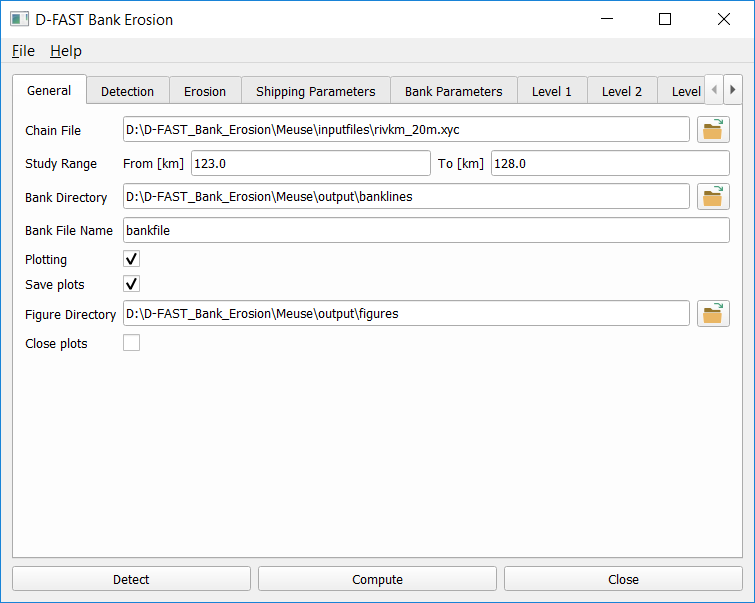
\includegraphics[width=12cm]{figures/gui1.png}
\caption{Example of \dfastbe graphical user interface}
\label{dfastbeGUI}
\end{figure}

All files and paths are shown using absolute paths in the graphical user interface, but they will be converted as much as possible to relative paths when saving the configuration to file.
The content of the first (General) and second (Detection) tabs are relevant for the bank line detection analysis.
All tabs except for the second (Detection) tab are relevant for the bank erosion analysis.

\section{Run mode 'banklines'}

When \dfastbe is run in this mode, it determines the representative bank lines within the area of interest; for background information see \autoref{Chp3}.
The input is given through the analysis configuration file, see \autoref{Sec2.4}.

When the configuration file has the name 'dfastbe.cfg' and is located in the work directory the program can be called as follows:

\begin{Verbatim}
dfastbe -mode banklines
\end{Verbatim}

If the definition file has another name the following call should be used:

\begin{Verbatim}
dfastbe -mode banklines -config path\other.cfg
\end{Verbatim}

with \command{path} the path to the directory where the configuration file is located and \command{other.cfg} the name of the configuration file.

Required input parameters:

\begin{itemize}
\item \dflowfm output file (netCDF map-file) at representative discharge (\command{SimFile}),
\item Number of bank Lines (\command{NBank} default two, the left and right bank),
\item For each of the bank lines a file with xy-coordinates of the search lines i.e. the approximate location of the bank line (\command{Line1}, \command{Line2}, ..., \command{LineN}, with $N$ the number of bank lines)
\item File which links river kilometres to xy-coordinates (\command{RiverKM}),
\end{itemize}

Output:

\begin{itemize}
\item XY-coordinates of the determined bank lines.
\item Plot of the bank lines (optional, \command{Plotting} and \command{SavePlots})
\end{itemize}

The computation has ended successfully when the message "BankLines ended successfully!" appears.

An example of the graphical output of the 'banklines' mode is shown in \autoref{Fig2.2}.
The water depth is given with colored surfaces (per grid cell), the black lines are the determined bank lines and the river kilometers are displayed along the river axis.

\Note To obtain the correct results, the search lines for the banks given by \command{Line1}, \command{Line2}, ..., \command{LineN} (obtained for example from the 'oeverlijnen' from Baseline data) should follow the actual bank line (to be detected) within a distance indicated by \command{DLines} (default 50 \unitbrackets{m}).
Large distances between the points -- and thus large deviations from the actual bank lines -- will result in inaccurate bank lines as the detection algorithm will not detect bank lines reaches outside the indicated area of interest.

\begin{figure}
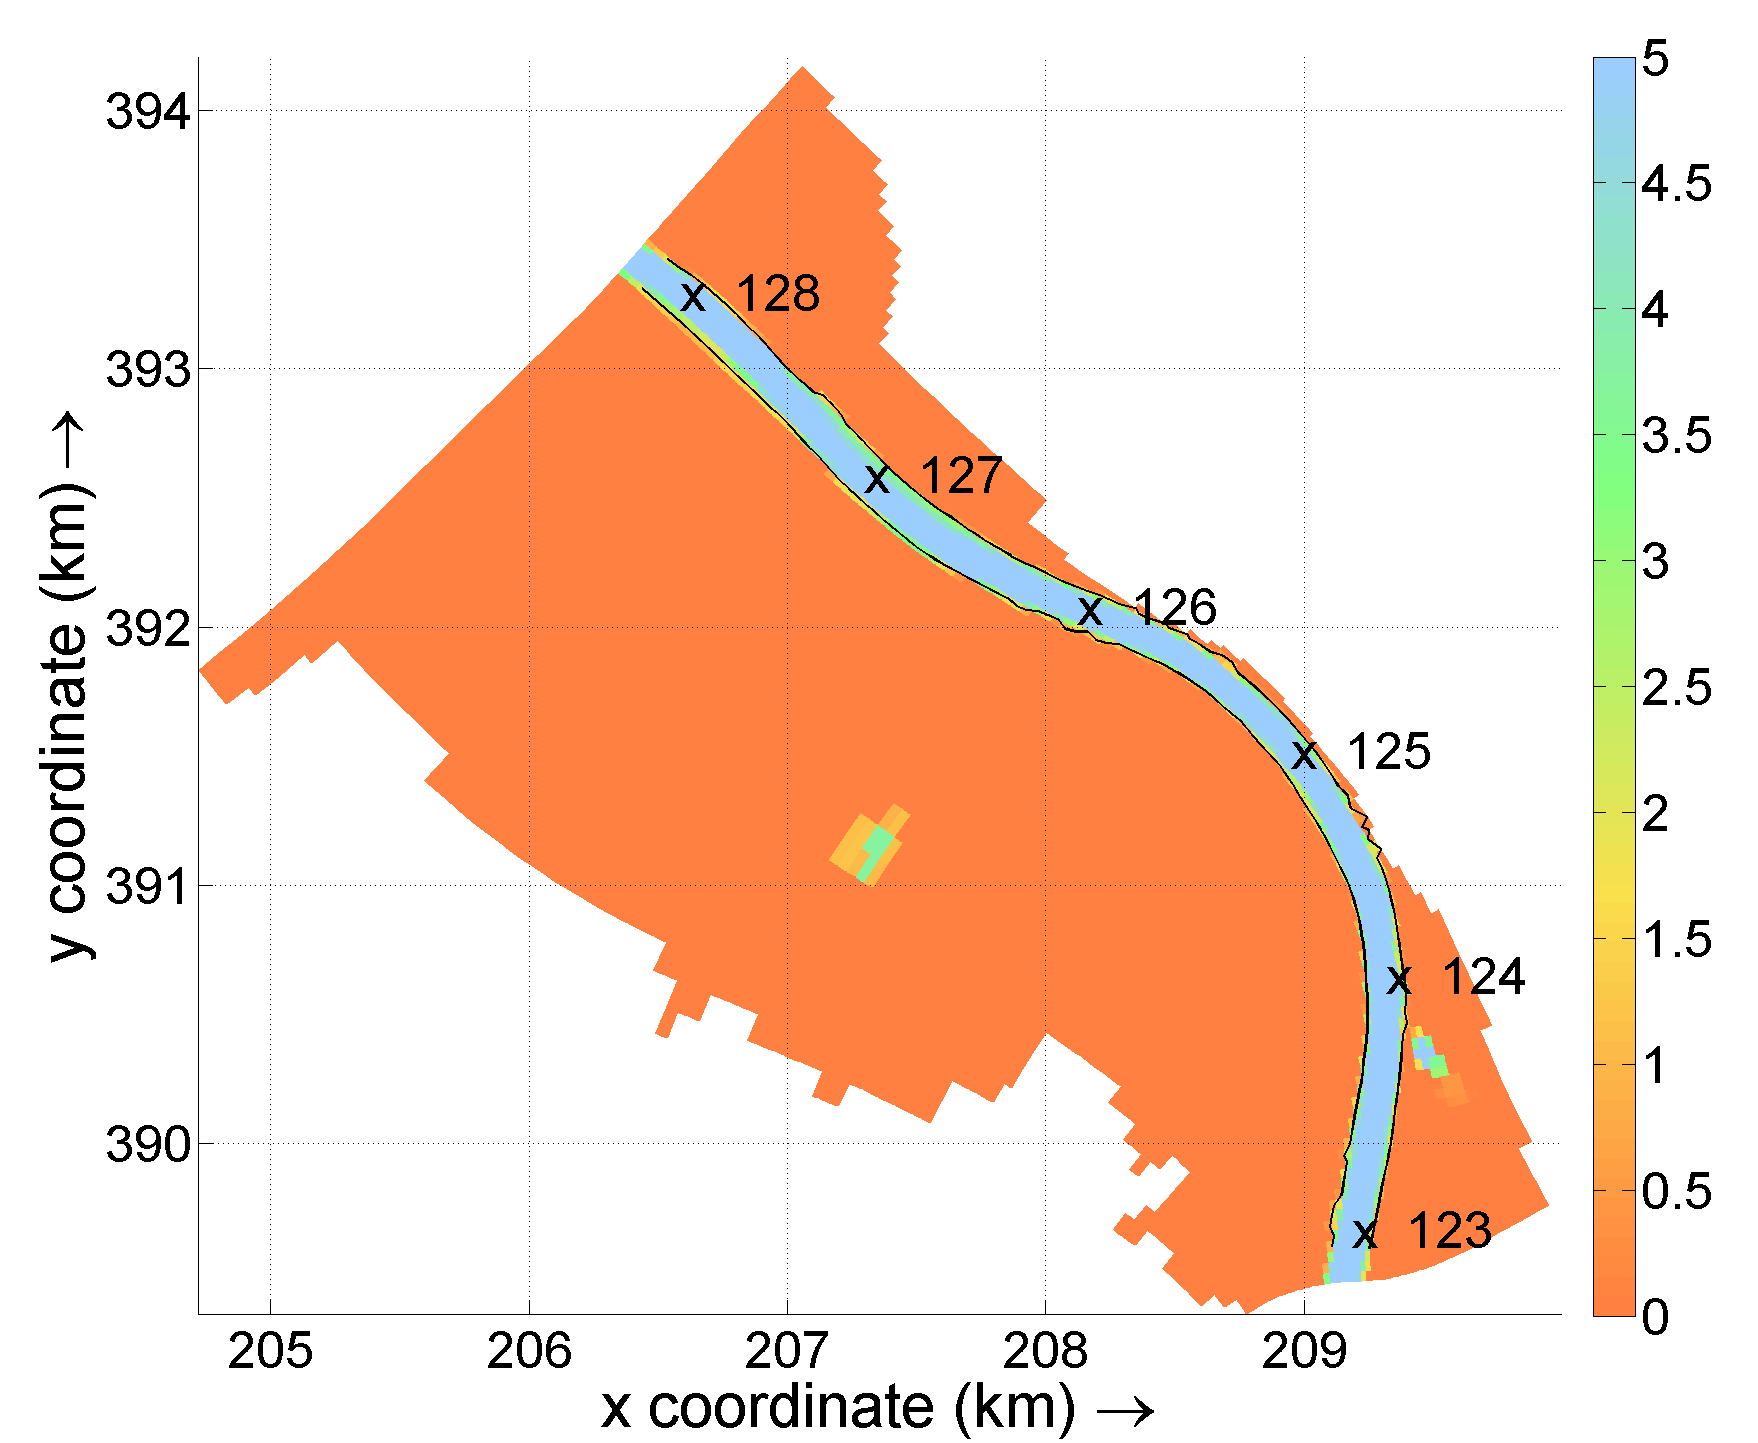
\includegraphics[width=\textwidth]{figures/Fig2-2.png}
\caption{Example of output of \dfastbe in 'banklines' mode}
\label{Fig2.2}
\end{figure}

\section{Run mode 'bankerosion'}

When \dfastbe is run in this mode, it determines the expected bank erosion within the area of interest; for background information see \autoref{Chp4}.
The input is given through the analysis configuration file, see \autoref{Sec2.4}.

When the configuration file has the name 'dfastbe.cfg' and is located in the work directory the program can be called as follows:

\begin{Verbatim}
dfastbe --mode bankerosion
\end{Verbatim}

If the configuration file has another name the following call should be used:

\begin{Verbatim}
dfastbe --mode bankerosion --config path\other.cfg
\end{Verbatim}

with \command{path} the path to the directory where the configuration file is located and \command{other.cfg} the name of the configuration file.

Required input:

\begin{itemize}
\item The period during which the bank erosion acts (\command{TErosion}, default 1 year),
\item The number of discharge levels (\command{NLevel}),
\item \dflowfm files (netCDF map-files) for the different discharge levels and the corresponding probability distribution (\command{SimFile1}, \command{SimFile2}, ..., \command{FileN} and \command{PDischarge1}, \command{PDischarge2}, ..., \command{PDischargeN}, with $N$ the number of discharge levels),
\item Number of bank Lines (\command{Nbank} default two, the left and right bank),
\item File which links river chainage (kilometres) to xy-coordinates (\command{RiverKM}),
\item XY-coordinates of the river and fairway axis (\command{RiverAxis}, \command{Fairway}),
\item Information about the strength or type of the soil of the banks (\command{BankType}).
This can be done either in the form of classes or with a critical shear stress (see \autoref{Tab4.1}).
In the first case \command{Classes} should be set to \command{true} and in the second case to \command{false} (default).
The bank strength information can be given either with a fixed value for the whole track or in a ASCII-file per river kilometer (first column river-km, second column bank type, see \autoref{Fig2.3}),
\item Shipping information (\command{Vship}, \command{Nship}, \command{ShipType}, \command{Draught}).
This can be done either with a fixed value for the whole track or in a file per river kilometer (first column river-km, second column shipping information: similar to entering bank type, see \autoref{Fig2.3}).
\end{itemize}

Output:

\begin{itemize}
\item Map with water depth, initial bank lines, river kilometers and fairway axis (see \autoref{Fig2.4}),
\item Map with erosion sensitivity of the banks based on computed bank retreat (see \autoref{Fig2.5}),
\item The computed erosion volume during the simulation period split up per bank (see \autoref{Fig2.6a}) and per discharge level (see \autoref{Fig2.6b}),
\item Total erosion volume based on equilibrium bank line (see \autoref{Fig2.7}),
\item Control figures for water levels of each discharge (see \autoref{Fig2.8} and \autoref{Fig2.9}),
\item Control figures for flow velocity of each discharge (see \autoref{Fig2.10} and \autoref{Fig2.11}),
\item Map with indication of applied bank type (see \autoref{Fig2.12}),
\item Bank retreat at the end of the simulation period and for the equilibrium situation (see \autoref{Fig2.13}),
\item XY-coordinates of the computed bank lines at the end of the simulation period and of the equilibrium bank lines.
\end{itemize}

The maps and graphs are only created when \command{Plotting} is on and written to file if \command{SavePlots} is on.
The computation has ended successfully when the message "Bank line detection ended successfully!" appears.

\begin{figure}
\begin{Verbatim}
  0.0          1
  75.2         3
  90.3         2
  110.0        0
  130.5        4
  153.1        3
  206.9        2
\end{Verbatim}
\caption{Example of input file for bank strength classes per river kilometer: from 0.0 - 75.2 km class 1, from 75.2 - 90.3 km class 3, etc.
When no information is available, the closest value will be used.}
\label{Fig2.3}
\end{figure}

\begin{figure}
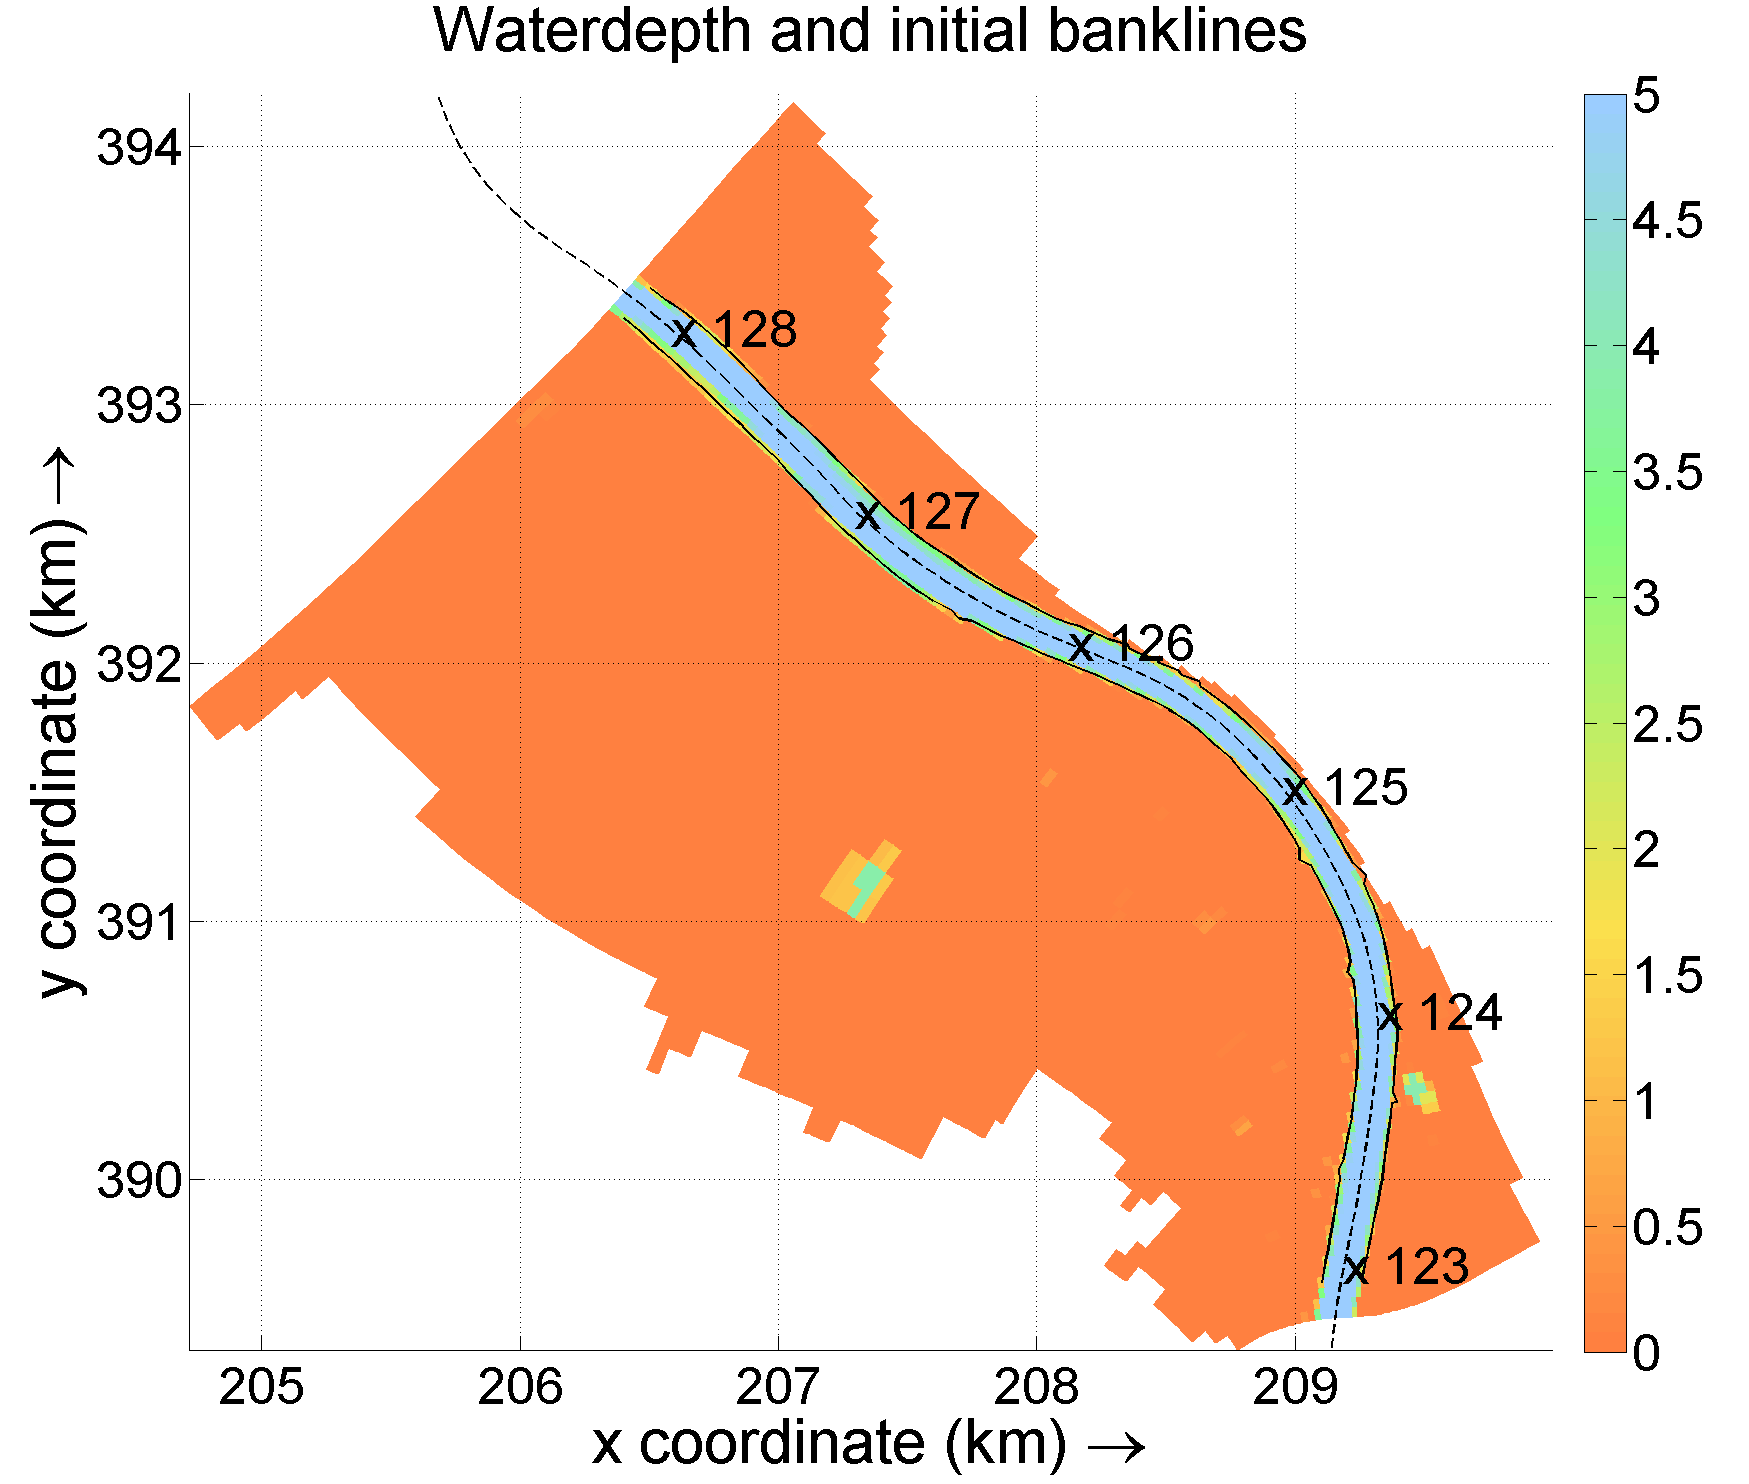
\includegraphics[width=\textwidth]{figures/Fig2-4.png}
\caption{Map of water depth, initial bank lines, river kilometers and fairway axis}
\label{Fig2.4}
\end{figure}

\begin{figure}
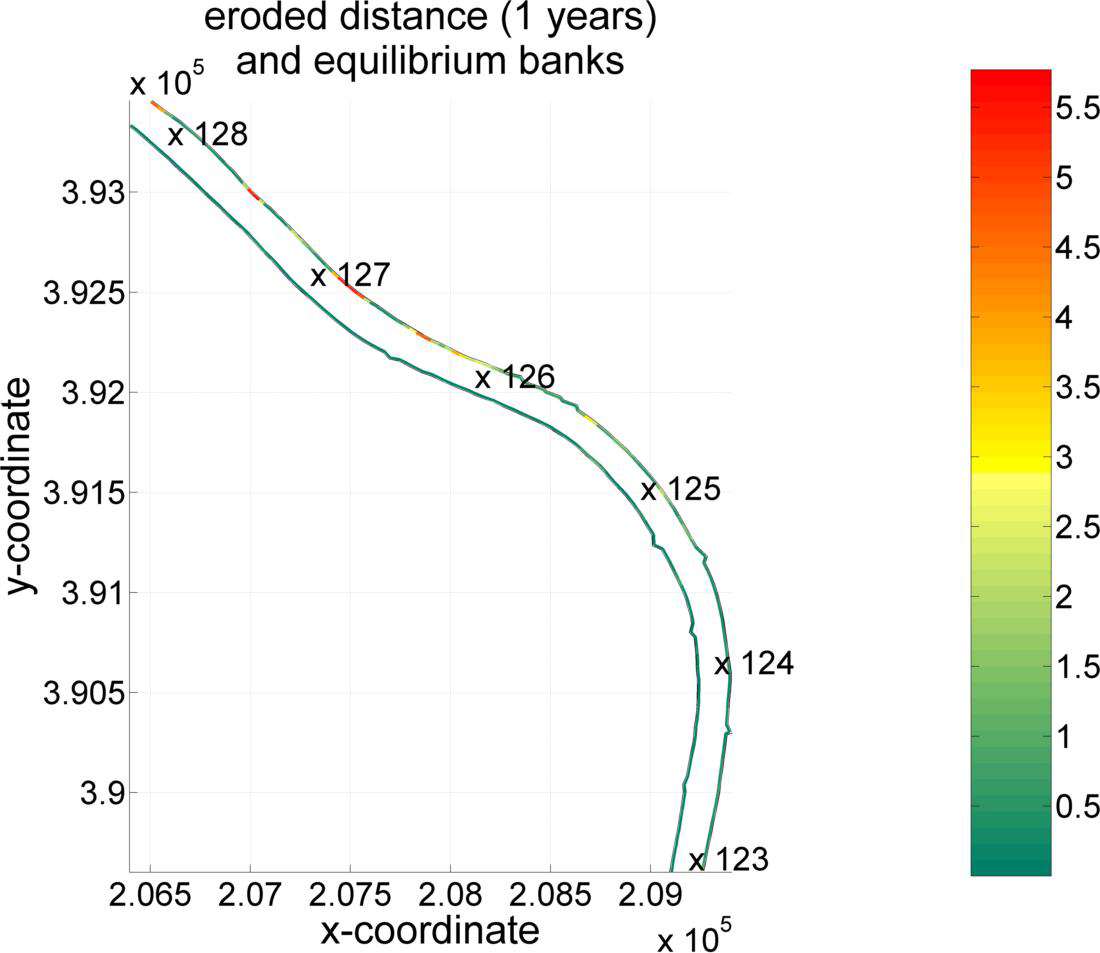
\includegraphics[width=\textwidth]{figures/Fig2-5.png}
\caption{Map of erosion sensitivity}
\label{Fig2.5}
\end{figure}

\begin{figure}
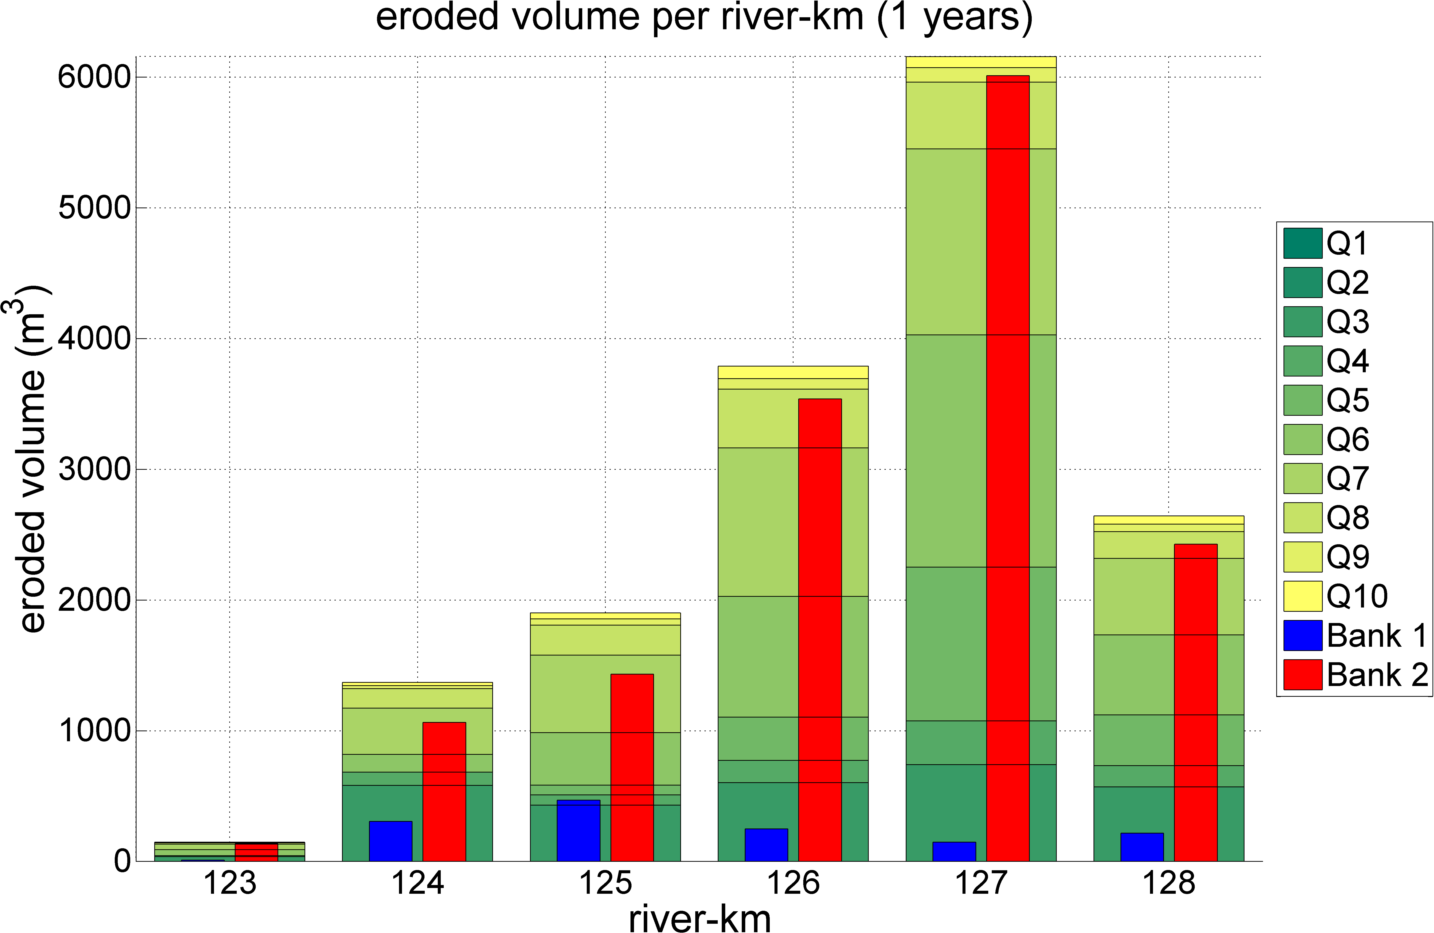
\includegraphics[width=\textwidth]{figures/Fig2-6.png}
\caption{Eroded volume subdivided per bank line}
\label{Fig2.6a}
\end{figure}

\begin{figure}
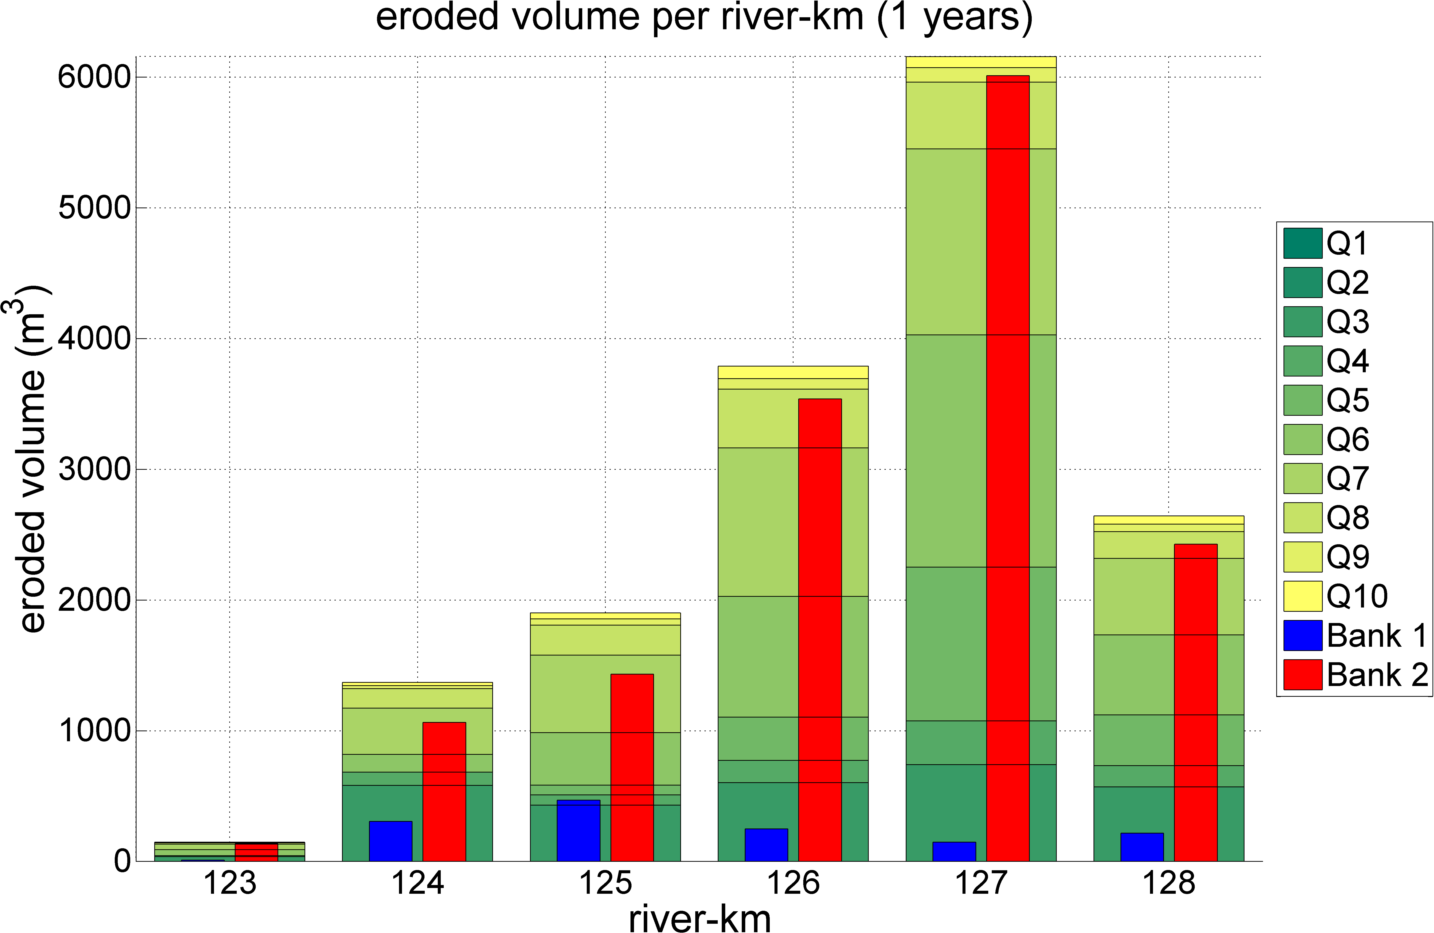
\includegraphics[width=\textwidth]{figures/Fig2-6.png}
\caption{Eroded volume subdivided per discharge level}
\label{Fig2.6b}
\end{figure}

\begin{figure}
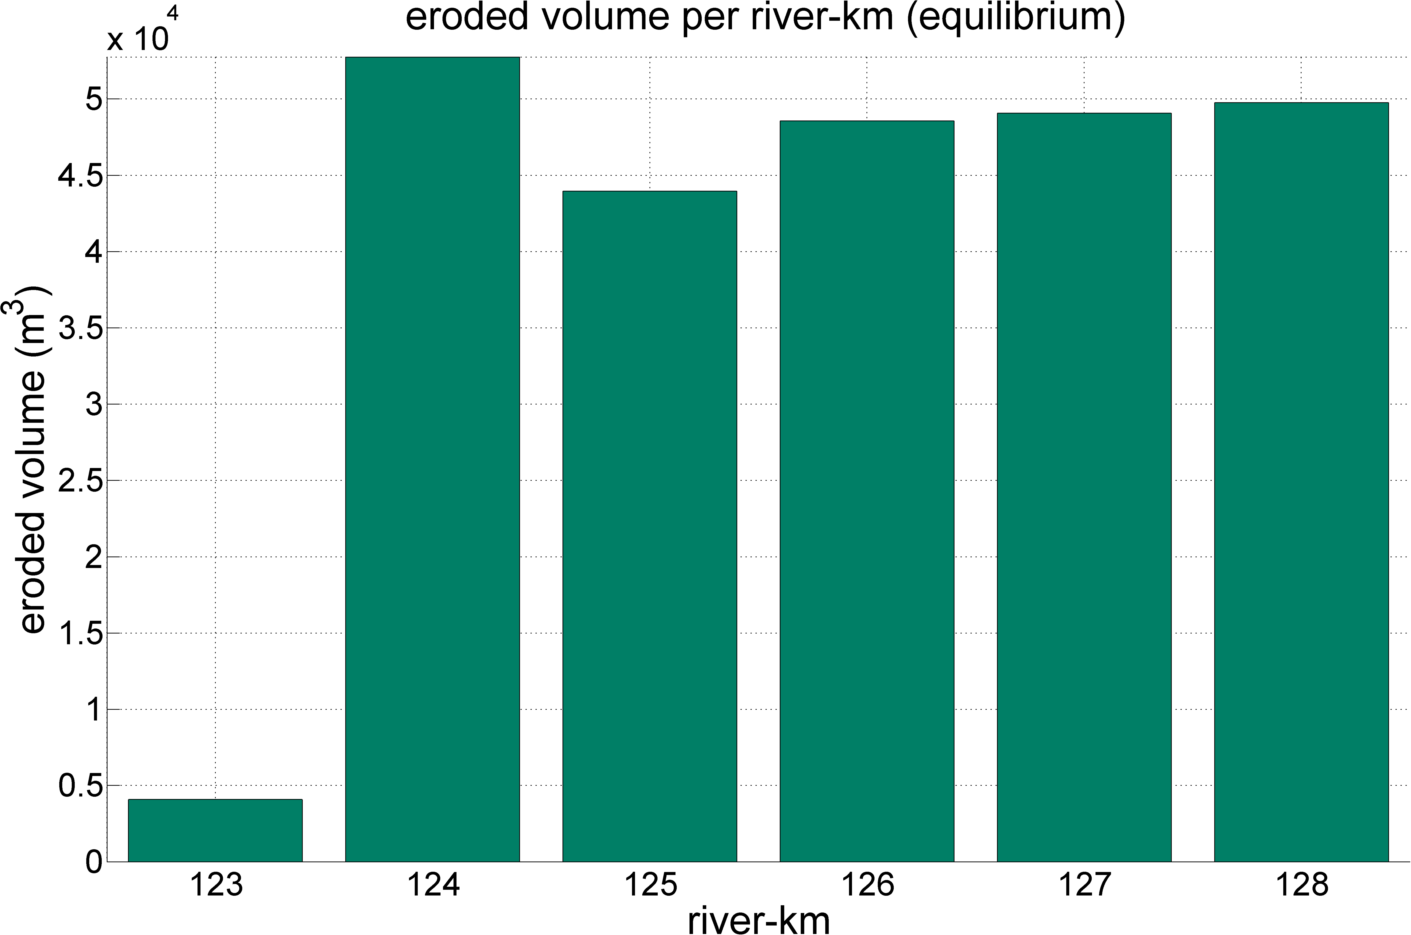
\includegraphics[width=\textwidth]{figures/Fig2-7.png}
\caption{Total erosion volume based on equilibrium bank line}
\label{Fig2.7}
\end{figure}

\begin{figure}
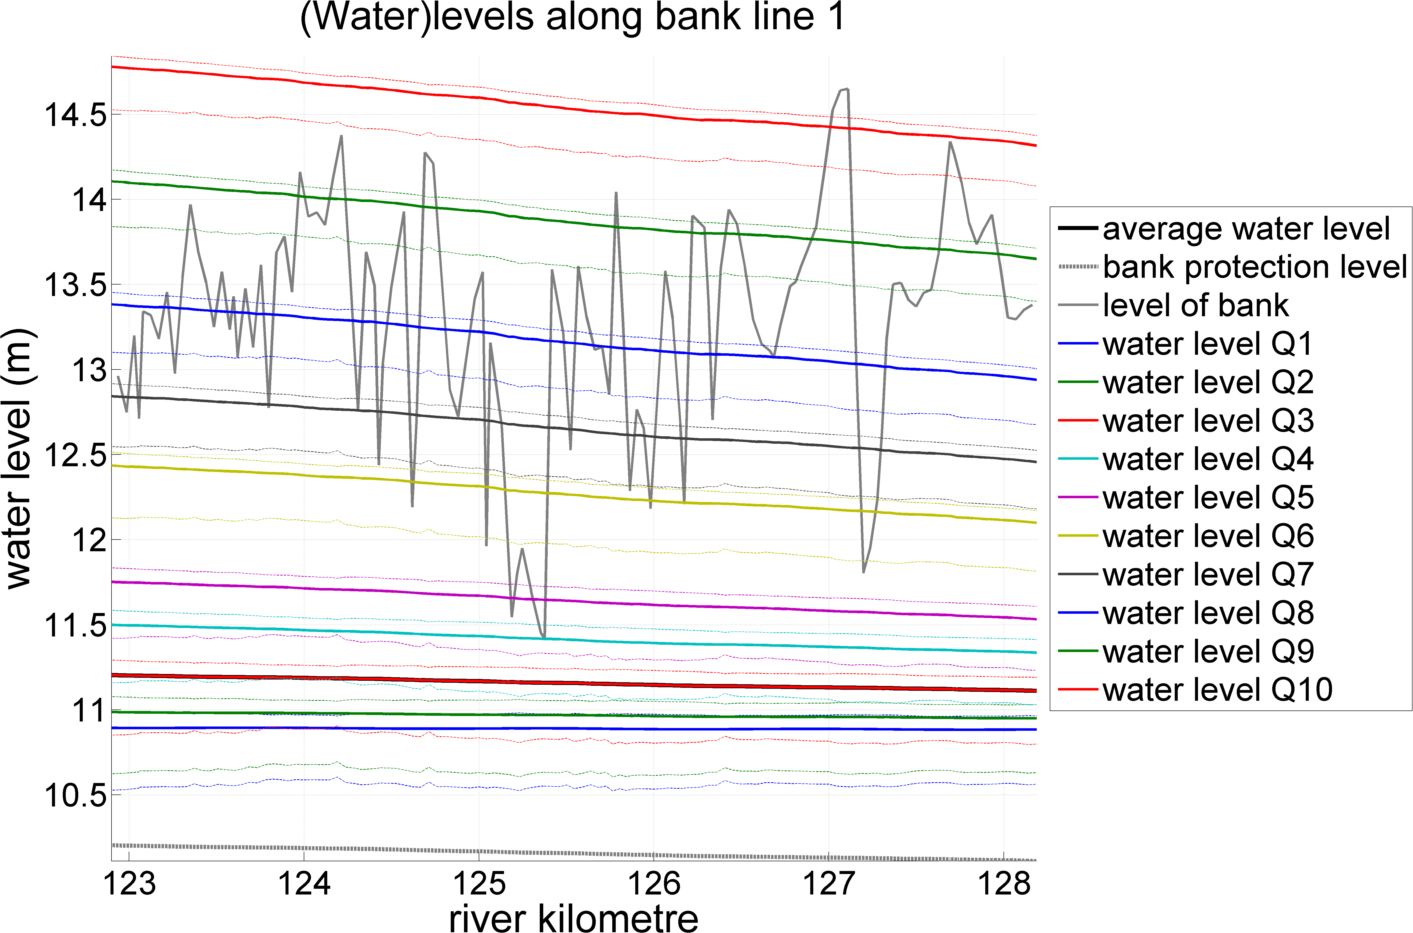
\includegraphics[width=\textwidth]{figures/Fig2-8.png}
\caption{Control figure for water levels of each discharge (bank line 1)}
\label{Fig2.8}
\end{figure}

\begin{figure}
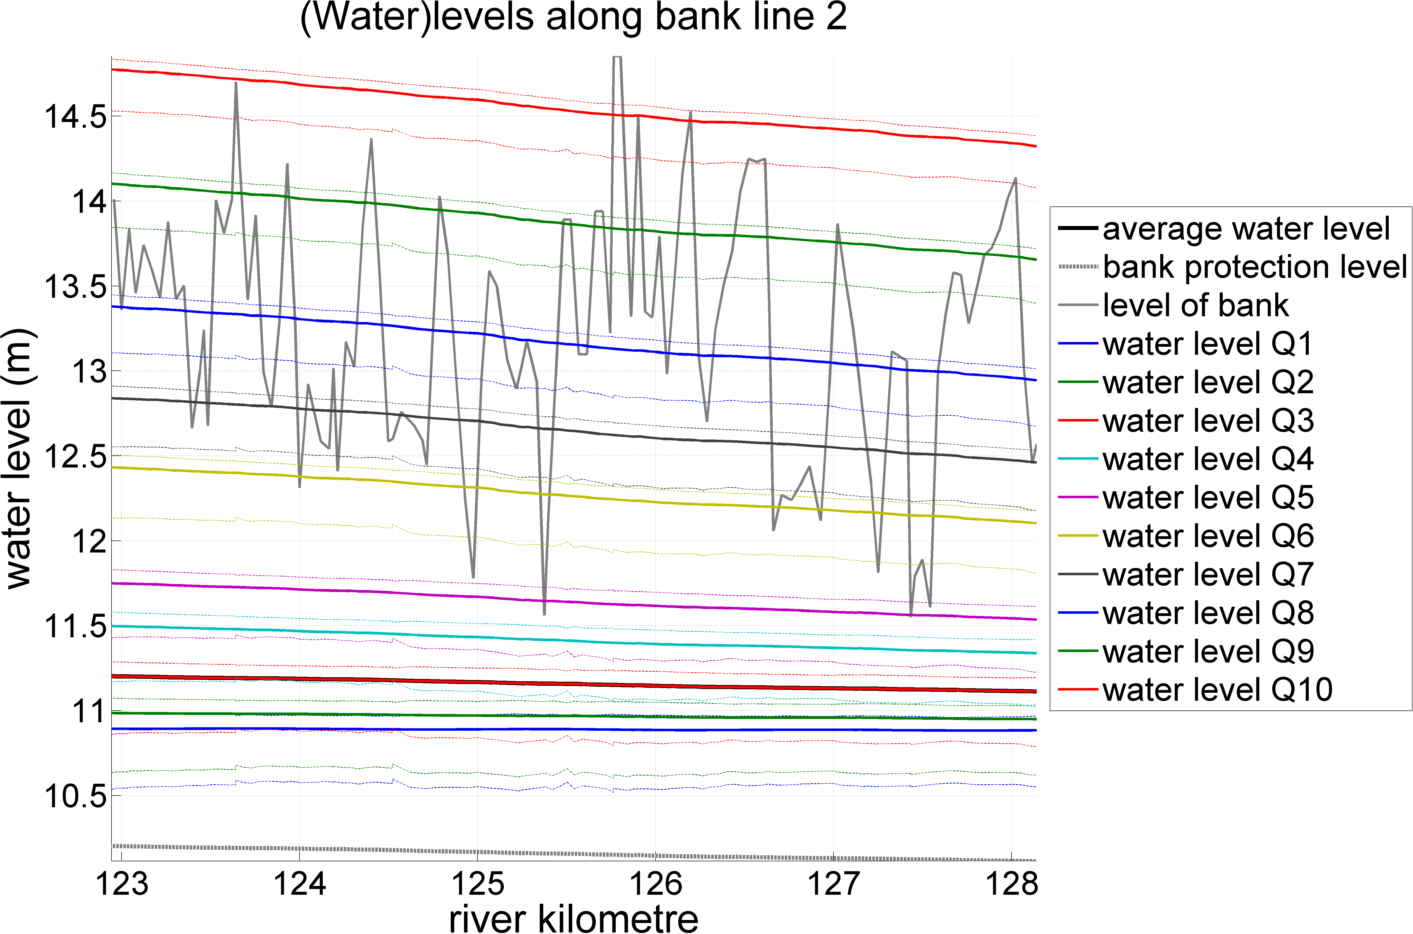
\includegraphics[width=\textwidth]{figures/Fig2-9.png}
\caption{Control figure for water levels of each discharge (bank line 2)}
\label{Fig2.9}
\end{figure}

\begin{figure}
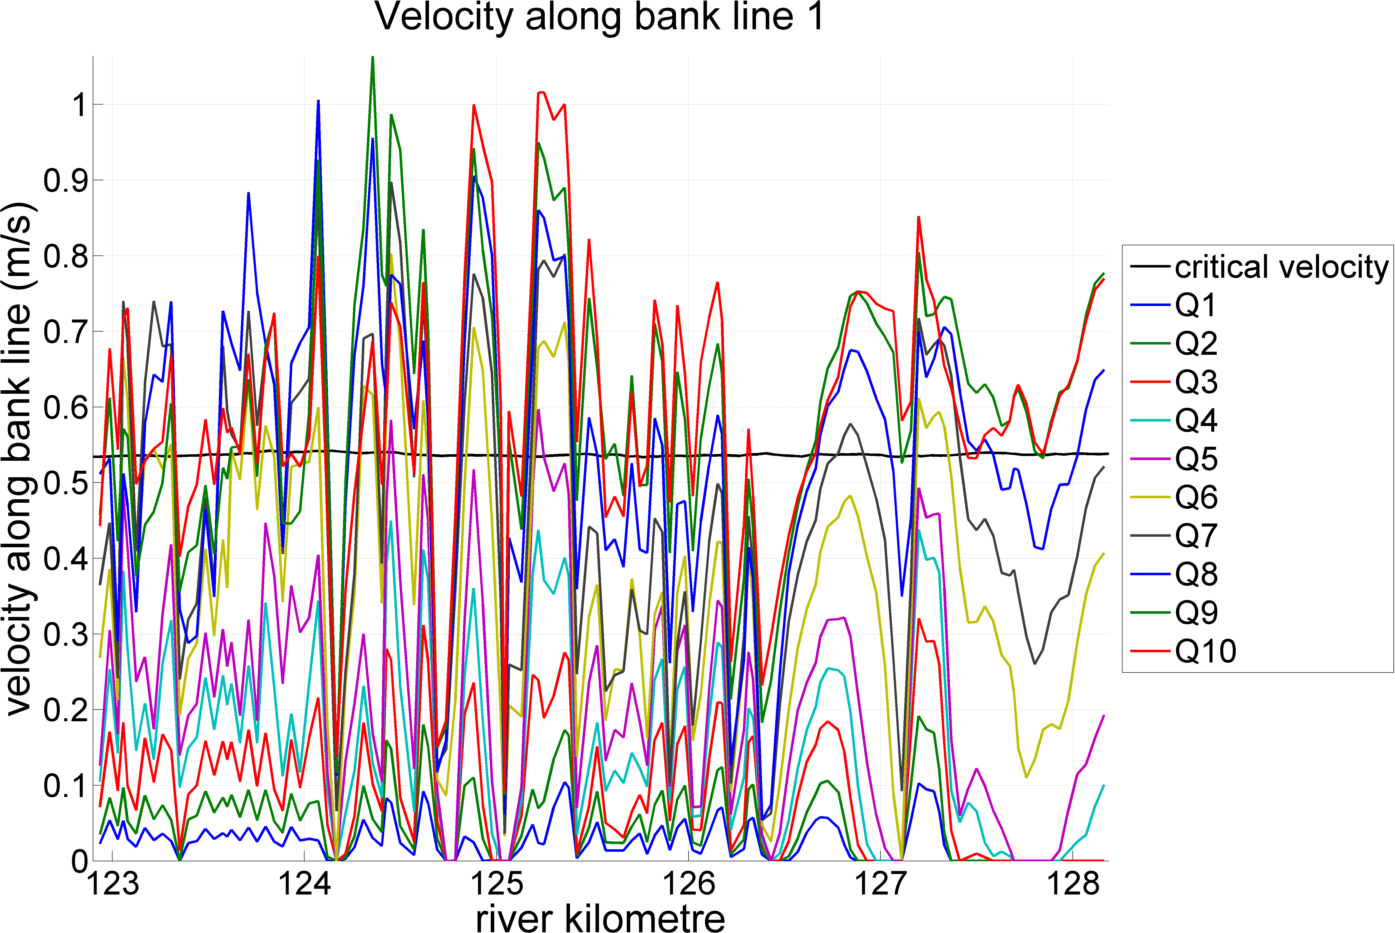
\includegraphics[width=\textwidth]{figures/Fig2-10.png}
\caption{Control figure for velocities of each discharge (bank line 1)}
\label{Fig2.10}
\end{figure}

\begin{figure}
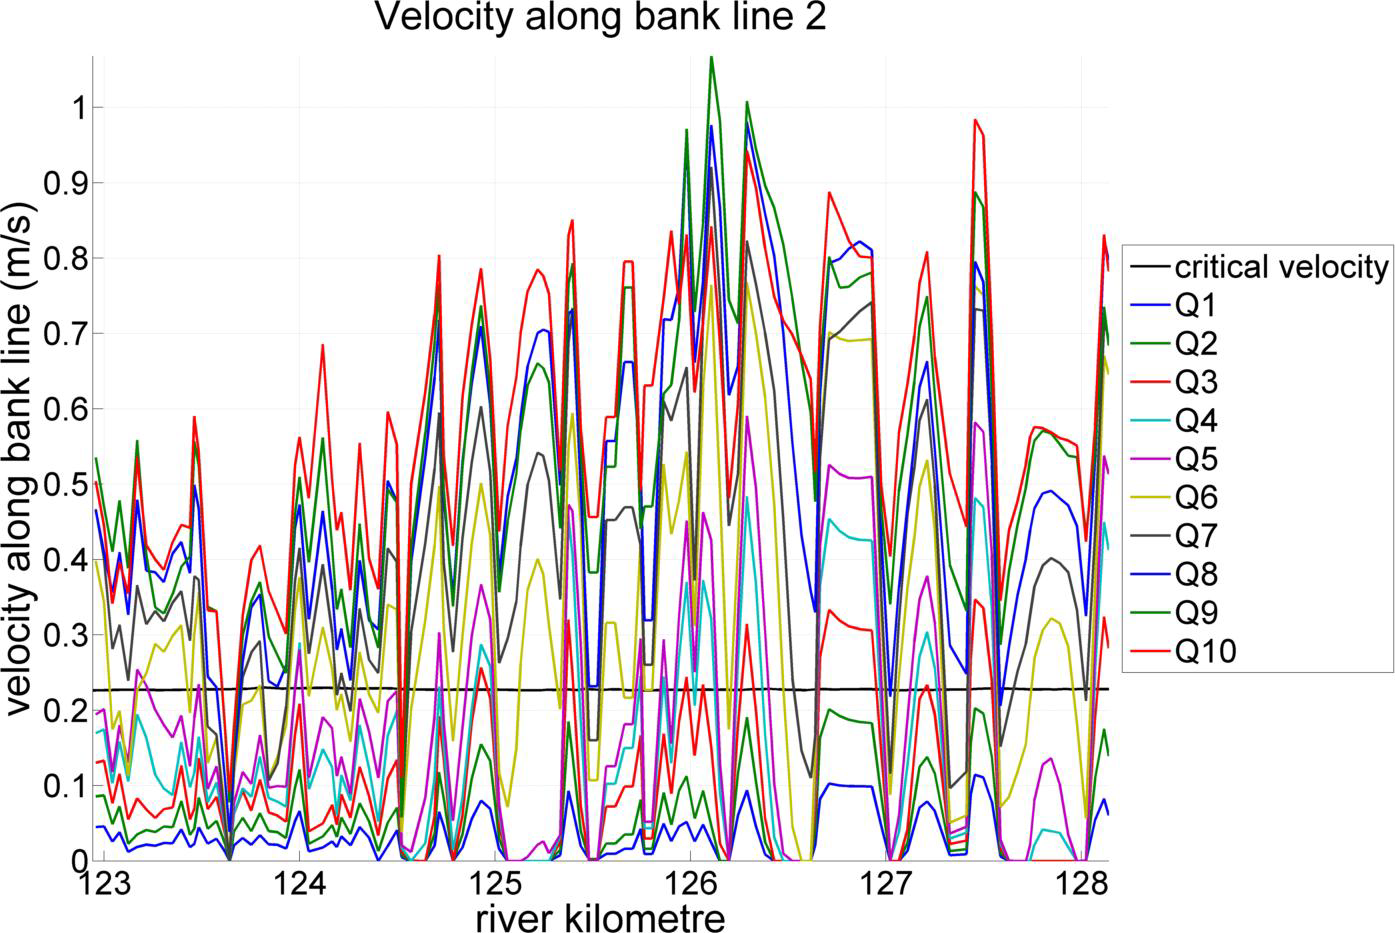
\includegraphics[width=\textwidth]{figures/Fig2-11.png}
\caption{Control figure for velocities of each discharge (bank line 2)}
\label{Fig2.11}
\end{figure}

\begin{figure}
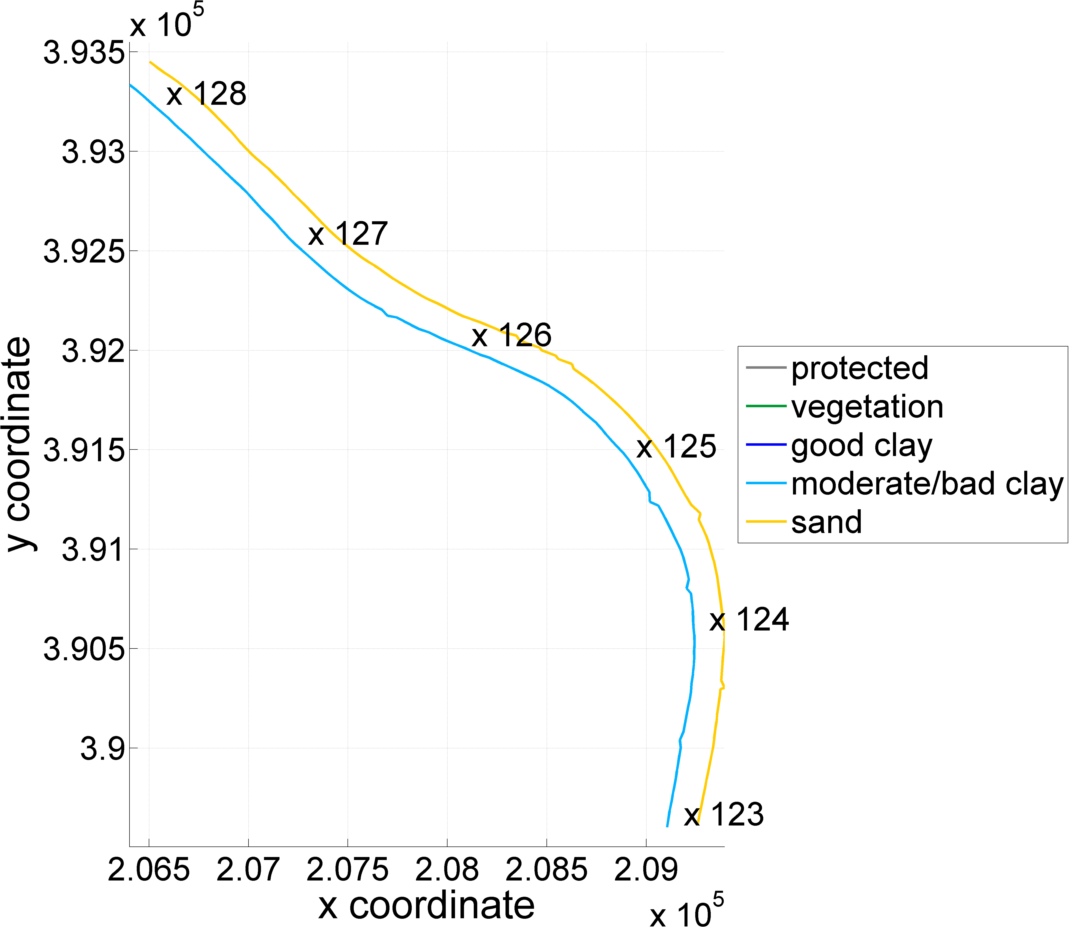
\includegraphics[width=\textwidth]{figures/Fig2-12.png}
\caption{Map with indication of applied bank type}
\label{Fig2.12}
\end{figure}

\begin{figure}
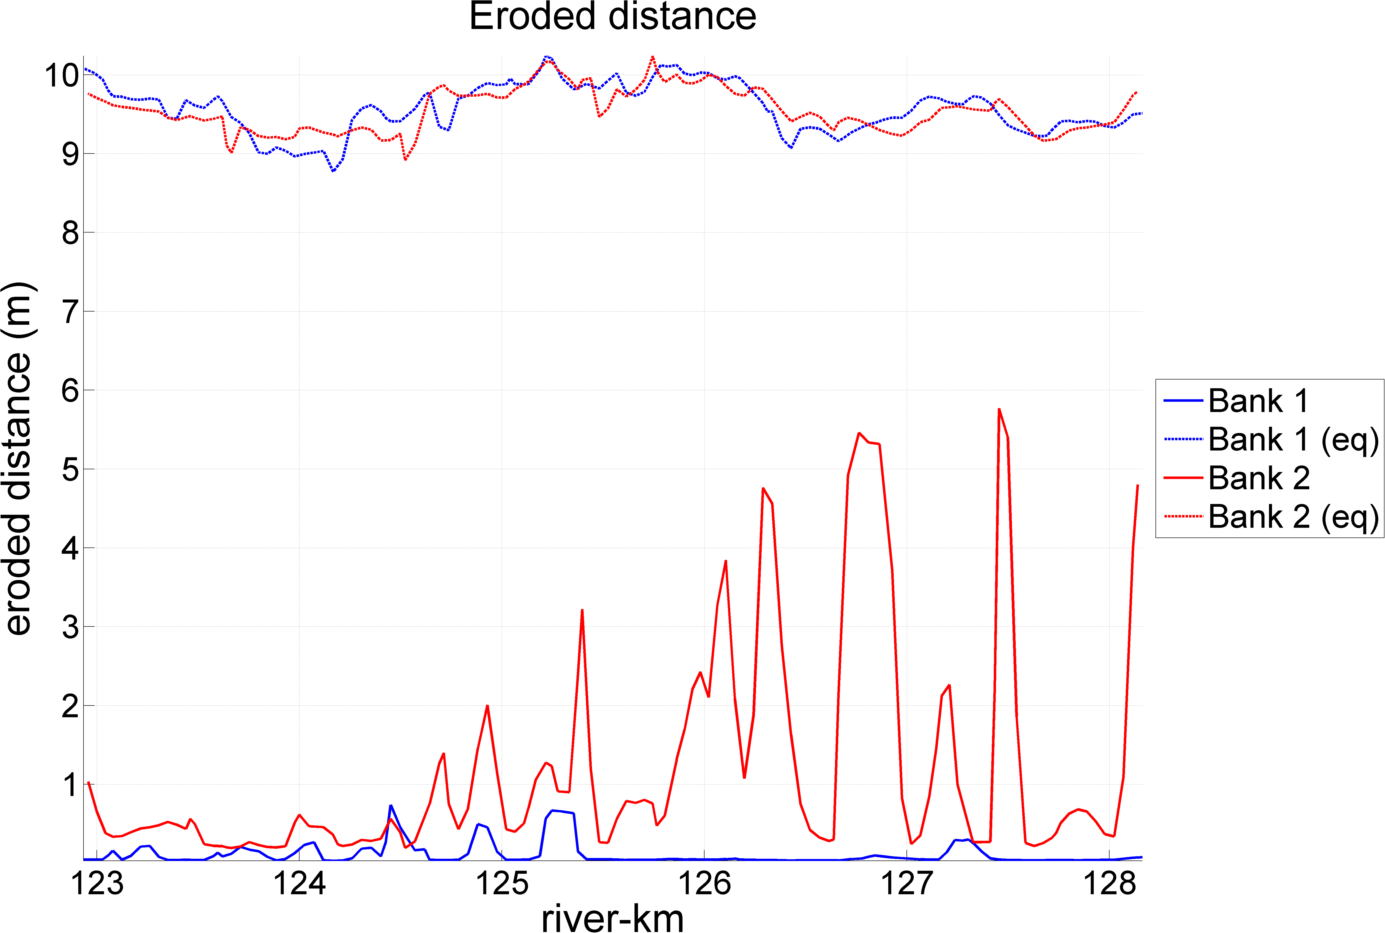
\includegraphics[width=\textwidth]{figures/Fig2-13.png}
\caption{Bank retreat at the end of the simulation period and for the equilibrium situation}
\label{Fig2.13}
\end{figure}

\section{Running from Python source code}
\dfastbe can also be run directly from the Python source code.
In that case the program can be started from the command prompt as

\begin{Verbatim}
python -m dfastbe.cmd ...options...
\end{Verbatim}

or from within a running Python environment as

\begin{Verbatim}
import dfastbe.cmd
dfastbe.cmd.cmd()
\end{Verbatim}

where optionally the \command{language} (default \command{UK}), \command{runmode} (default \command{GUI}) and \command{configfile} (default \command{dfastbe.cfg}) can be specified as arguments.